\documentclass[sectionformat = exercise]{gadsescript}

\settitle{Exercise Sheet 4}
\setsubtitle{Elias Gestrich}

\begin{document}
\maketitle

\section{Graphs}
\begin{enumerate}[label=\alph*)]
	\item ~\\
		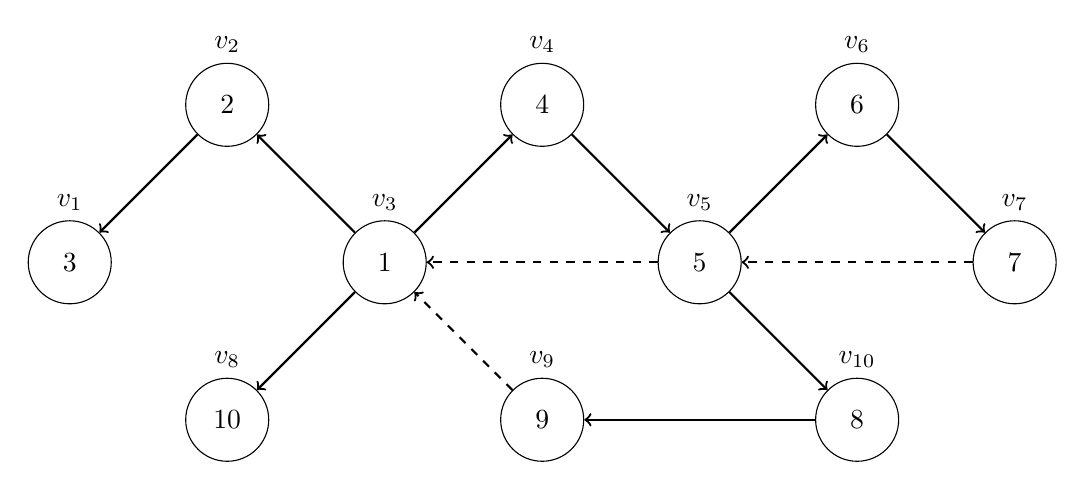
\begin{tikzpicture}
			\node (v1) [draw, circle, label=above: $v_1$, inner sep = 0, minimum size = 30] at (0,0) {$3$};
			\node (v2) [draw, circle, label=above: $v_2$, inner sep = 0, minimum size = 30] at (2,2) {$2$};
			\node (v3) [draw, circle, label=above: $v_3$, inner sep = 0, minimum size = 30] at (4,0) {$1$};
			\node (v4) [draw, circle, label=above: $v_4$, inner sep = 0, minimum size = 30] at (6,2) {$4$};
			\node (v5) [draw, circle, label=above: $v_5$, inner sep = 0, minimum size = 30] at (8,0) {$5$};
			\node (v6) [draw, circle, label=above: $v_6$, inner sep = 0, minimum size = 30] at (10,2) {$6$};
			\node (v7) [draw, circle, label=above: $v_7$, inner sep = 0, minimum size = 30] at (12,0) {$7$};
			\node (v8) [draw, circle, label=above: $v_8$, inner sep = 0, minimum size = 30] at (2,-2) {$10$};
			\node (v9) [draw, circle, label=above: $v_9$, inner sep = 0, minimum size = 30] at (6,-2) {$9$};
			\node (v10) [draw, circle, label=above: $v_{10}$, inner sep = 0, minimum size = 30] at (10,-2) {$8$};
			\draw[->, thick] (v3) -- (v2);
			\draw[->, thick] (v2) -- (v1);
			\draw[->, thick] (v3) -- (v4);
			\draw[->, thick] (v4) -- (v5);
			\draw[->, thick, dashed] (v5) -- (v3);
			\draw[->, thick] (v5) -- (v6);
			\draw[->, thick] (v6) -- (v7);
			\draw[->, thick, dashed] (v7) -- (v5);
			\draw[->, thick] (v5) -- (v10);
			\draw[->, thick] (v10) -- (v9);
			\draw[->, thick, dashed] (v9) -- (v3);
			\draw[->, thick] (v3) -- (v8);
		\end{tikzpicture}
	\item ~\\
		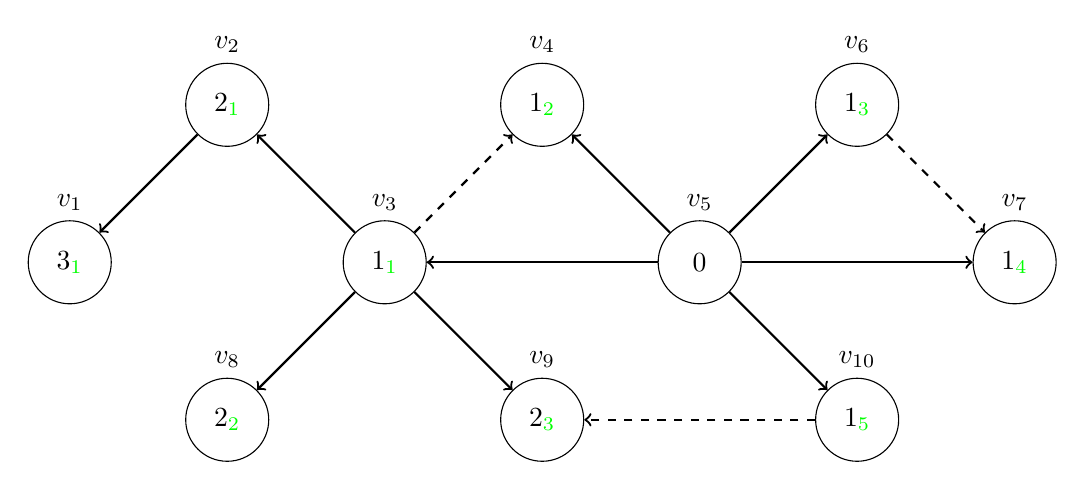
\begin{tikzpicture}
			\node (v1) [draw, circle, label=above: $v_1$, inner sep = 0, minimum size = 30] at (0,0) {$3_{\color{green}1}$};
			\node (v2) [draw, circle, label=above: $v_2$, inner sep = 0, minimum size = 30] at (2,2) {$2_{\color{green}1}$};
			\node (v3) [draw, circle, label=above: $v_3$, inner sep = 0, minimum size = 30] at (4,0) {$1_{\color{green}1}$};
			\node (v4) [draw, circle, label=above: $v_4$, inner sep = 0, minimum size = 30] at (6,2) {$1_{\color{green}2}$};
			\node (v5) [draw, circle, label=above: $v_5$, inner sep = 0, minimum size = 30] at (8,0) {$0$};
			\node (v6) [draw, circle, label=above: $v_6$, inner sep = 0, minimum size = 30] at (10,2) {$1_{\color{green}3}$};
			\node (v7) [draw, circle, label=above: $v_7$, inner sep = 0, minimum size = 30] at (12,0) {$1_{\color{green}4}$};
			\node (v8) [draw, circle, label=above: $v_8$, inner sep = 0, minimum size = 30] at (2,-2) {$2_{\color{green}2}$};
			\node (v9) [draw, circle, label=above: $v_9$, inner sep = 0, minimum size = 30] at (6,-2) {$2_{\color{green}3}$};
			\node (v10) [draw, circle, label=above: $v_{10}$, inner sep = 0, minimum size = 30] at (10,-2) {$1_{\color{green}5}$};
			\draw[->, thick] (v5) -- (v3);
			\draw[->, thick] (v5) -- (v4);
			\draw[->, thick] (v5) -- (v6);
			\draw[->, thick] (v5) -- (v7);
			\draw[->, thick] (v5) -- (v10);
			\draw[->, thick] (v3) -- (v2);
			\draw[->, thick, dashed] (v3) -- (v4);
			\draw[->, thick] (v3) -- (v8);
			\draw[->, thick] (v3) -- (v9);
			\draw[->, thick, dashed] (v6) -- (v7);
			\draw[->, thick, dashed] (v10) -- (v9);
			\draw[->, thick] (v2) -- (v1);

		\end{tikzpicture}
\end{enumerate}

\section{Iteration}
\begin{enumerate}[label=\alph*)]
	\item $[E, N, S, I, R, T]$\\$[E, I, S, N, R, T]$\\$[E, I, N, S, R, T]$\\$[E, I, N, R, S, T]$\\$[E, I, N, R, S, T]$
	\item \textit{SelectionSort} will sort $[2, 2, 1]$, so that the first $2$ will be after the second $2$.
	\item
		$[E, S, L, E, C, T]$\\
		$[E, L, S, E, C, T]$\\
		$[E, L, E, S, C, T]$\\
		$[E, E, L, S, C, T]$\\
		$[E, E, L, C, S, T]$\\
		$[E, E, C, L, S, T]$\\
		$[E, C, E, L, S, T]$\\
		$[C, E, E, L, S, T]$\\
		$[C, E, E, L, S, T]$\\
\end{enumerate}

\end{document}
